\documentclass{standalone}

\usepackage{tikz}
\usepackage{circuitikz}

\tikzset{block/.style = {draw, fill=white, very thick, rectangle, minimum height=1cm, minimum width=2cm},
         lblock/.style={draw,fill=white,very thick, rectangle, minimum height=3cm, minimum width=1cm},
         sum/.style= {draw, fill=white, very thick, circle, node distance=0.5cm}}

         
\begin{document}
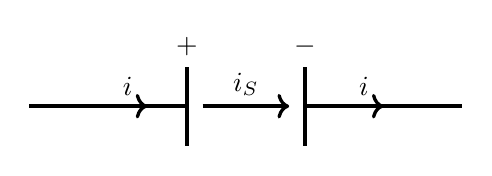
\begin{tikzpicture}[scale=2]
    \draw[-,very thick](-0.75,0)--(0.25,0);
    \draw[-,ultra thick](0.25,-0.25)--(0.25,0.25)node[above]{$+$};
    \draw[-, very thick](1,0)--(2,0);
    \draw[-,ultra thick](1,-0.25)--(1,0.25)node[above]{$-$};

    \draw[->,very thick](-0.25,0)--(0,0)node[midway,above]{$i$};
    \draw[->,very thick](1.25,0)--(1.5,0)node[midway,above]{$i$};
    \draw[->,very thick](0.35,0)--(0.9,0)node[midway,above]{$i_S$};
\end{tikzpicture}
\end{document}